%%%%%%%%%%%%%%%%%%%%%%%%%%%%%%%%%%%%%%
%%%%%%%%%%%%%%%%%%%%%%%%%%%%%%%%%%%%%%
% Do not edit the TeX file your work
% will be overwritten.  Edit the RnW
% file instead.
%%%%%%%%%%%%%%%%%%%%%%%%%%%%%%%%%%%%%%
%%%%%%%%%%%%%%%%%%%%%%%%%%%%%%%%%%%%%%



We consider the problem of clustering time-course gene expression data. 
While thousands of genes might be simultaneously 
measured in a given genomics experiment, 
many genes may exhibit similar expression patterns.  
Clustering gene expressions
is one way to reduce the dimensionality of a complex data set 
and to facilitate scientific interpretations of intricate biological processes. 
Often, such dimensionality reduction is used for exploratory analysis and
is a first step before further downstream investigation.  
It is important, therefore, to ascertain the stability of the 
discovered clusters. 
 
We study a publicly available data set of mice gene expression
\citep{shoemaker:2015:ultrasensitive}.
Mice were infected with influenza virus,
and expression levels of a set of genes were assessed at 14 time points after infection.
Three measurements were taken at each time point (called biological replicates), 
for a total of $\ntimepoints = 42$ measurements per gene. 

\subsubsection*{The model}
Let $\x_\n\in\mathbb{R}^\ntimepoints$ be measurments of gene $\n$
at $\ntimepoints$ time points.
Following \citet{Luan:2003:clustering} we apply cubic B-splines to 
smooth the time course expression data.
Let $\regmatrix$ be the $\ntimepoints \times \d$ B-spline regressor matrix; 
that is, the $ij$-th entry of $\regmatrix$
is the $j$-th B-spline basis vector evaluated at the
$i$-th time point. 
\figref{example_genes} shows measurements from an example gene and 
the B-spline basis. 

In this model, 
each component is characterized by a vector of regression coefficients
$\mu_\k$ and a variance $\tau^{-1}_\k$, so
$\beta_k = (\mu_\k, \tau_\k)$.
The distribution of the data arising from component $k$ is
\begin{align}\eqlabel{mice_model}
\p(\x_\n | \beta_\k, \b_\n) =
\normdist{\x_\n | \regmatrix\mu_\k + \b_\n,
\tau_\k^{-1}I_{\ntimepoints \times \ntimepoints}},
\end{align}
%
where $\b_\n$ is a gene-specific additive offset and $I$ is the identity matrix.
We include the additive offset because we
are interested in clustering gene expressions based on their patterns over time,
not their absolute level.

The mixture weights $\pi$ and cluster assignments $\z$ are drawn from the 
stick-breaking process described in \secref{model_bnp}. 

Our variational approximation factorizes similarly to \eqref{vb_mf}
except with an additional factor for the additive shift. 
In our variational approximation, we also make a simplification by letting
$\q(\beta_\k \vert \eta) = \delta (\beta_k \vert \eta)$, 
where $\delta(\cdot \vert \eta)$ denotes a point mass at a parameterized location. 
See \appref{app_mice} for further details concerning the model and
variational approximation. 


\begin{knitrout}
\definecolor{shadecolor}{rgb}{0.969, 0.969, 0.969}\color{fgcolor}\begin{figure}[!h]

{\centering 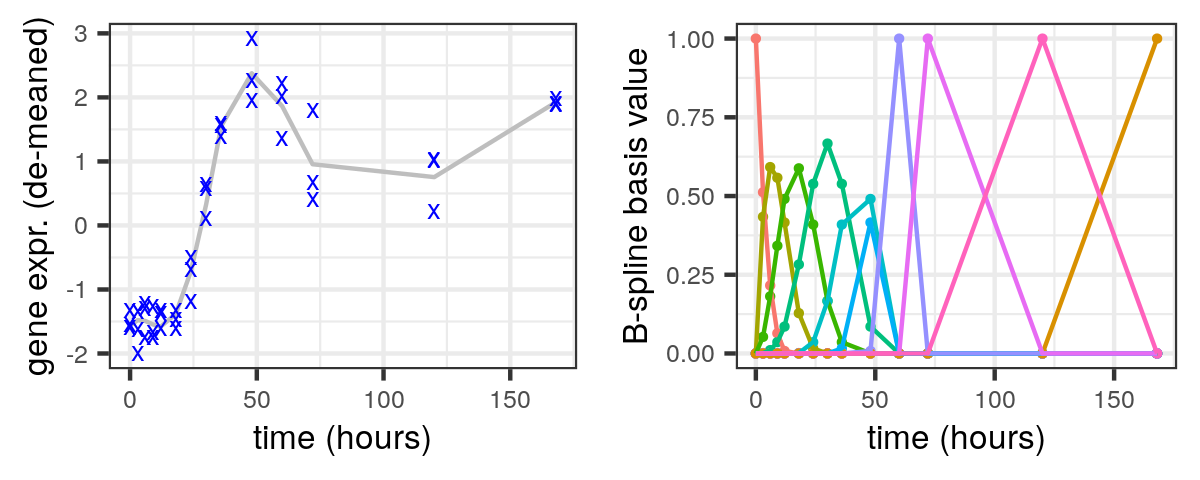
\includegraphics[width=0.980\linewidth,height=0.392\linewidth]{figure/example_genes-1} 

}

\caption[(Left) An example gene and its expression measured at 14 unique time points
    with three biological replicates at each time point.
     (Right) The cubic B-spline basis with 7 degrees of freedom, 
    along with three indicator functions for the last three time points, 
    $\timeindx = 72, 120, 168$]{(Left) An example gene and its expression measured at 14 unique time points
    with three biological replicates at each time point.
     (Right) The cubic B-spline basis with 7 degrees of freedom, 
    along with three indicator functions for the last three time points, 
    $\timeindx = 72, 120, 168$.}\label{fig:example_genes}
\end{figure}


\end{knitrout}
%

In this application, we expect to uncover finer structure, 
so we start with a larger $\alpha$ than the previous example 
and set $\alpha_0 = 6$ in the initial GEM prior. 
\figref{gene_initial_coclustering} displays the inferred co-clustering matrix
at this choice of $\alpha_0$. 
More precisely, let $\gcoclustering(\eta)\in\mathbb{R}^{\N\times\N}$ 
denote the co-clustering matrix, 
whose $(i,j)$-th entry is the
posterior probability that gene $i$ belongs to the same cluster
as gene $j$, given by 
\begin{align*}
[\gcoclustering(\eta)]_{ij}
&= \expect{\q(\z\vert\eta)}{\ind{\z_{i} = \z_{j}}} \\
&= \sum_{k=1}^{\kmax}\left(\expect{\q(\z_i\vert\eta)}{\z_{ik}}
\expect{\q(\z_j\vert\eta)}{\z_{jk}}\right).
\end{align*}

% $\gcoclustering(\eta)$, whose , given by 
% \begin{align*}
% \gcoclustering{ij}(\eta) 
% &= \expect{\q(\z\vert\eta)}{\ind{\z_{i} = \z_{j}}} \\
% &= \sum_{k=1}^{\kmax}\left(\expect{\q(\z_i\vert\eta)}{\z_{ik}}
% \expect{\q(\z_j\vert\eta)}{\z_{jk}}\right).
% \end{align*}

Below, we evaluate the sensitivity of the inferred co-clustering matrix to 
both parametric and functional perturbations to the stick distribution. 

\newcommand{\MiceSmoothers}{
% moving this to appendix 

\begin{knitrout}
\definecolor{shadecolor}{rgb}{0.969, 0.969, 0.969}\color{fgcolor}\begin{figure}[!h]

{\centering 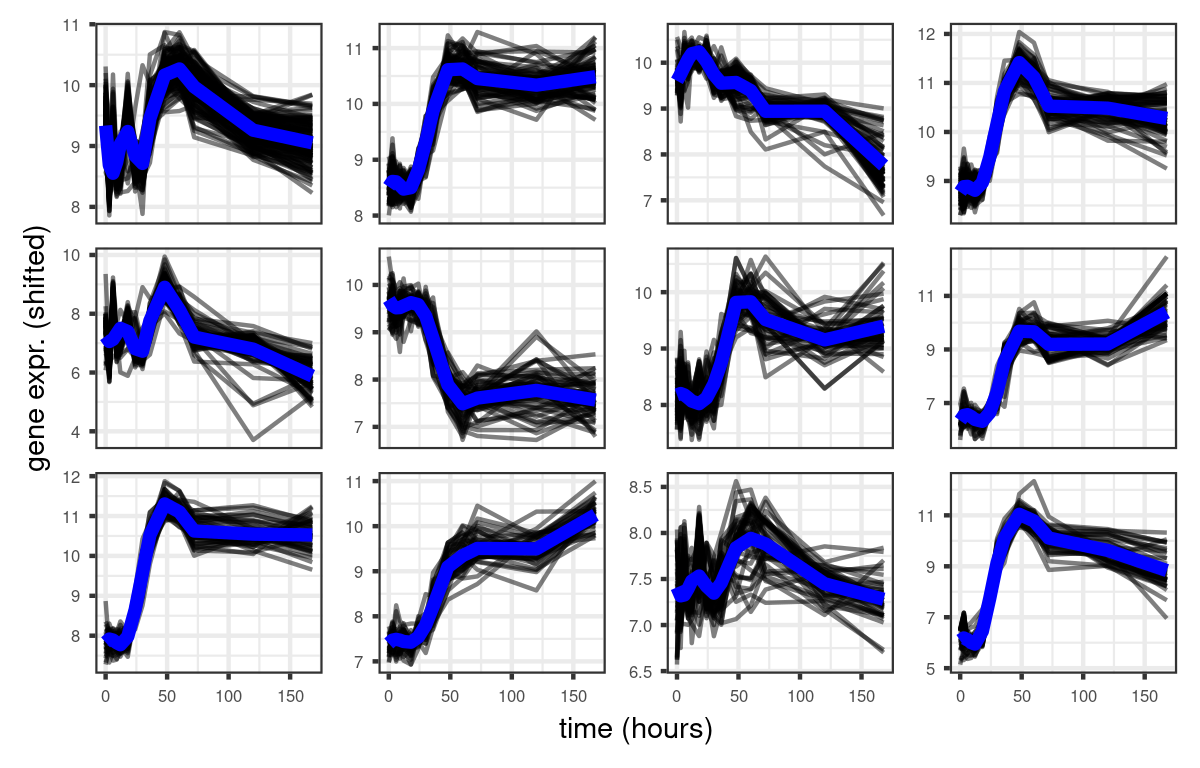
\includegraphics[width=0.980\linewidth,height=0.627\linewidth]{figure/gene_centroids-1} 

}

\caption[Inferred clusters in the mice gene expression dataset]{Inferred clusters in the mice gene expression dataset. 
    Shown are the twelve most occupied clusters. 
    In blue, the inferred cluster centroid. 
    In grey, gene expressions averaged over replicates and
    shifted by their inferred intercepts. }\label{fig:gene_centroids}
\end{figure}


\end{knitrout}
}



\begin{knitrout}
\definecolor{shadecolor}{rgb}{0.969, 0.969, 0.969}\color{fgcolor}\begin{figure}[!h]

{\centering 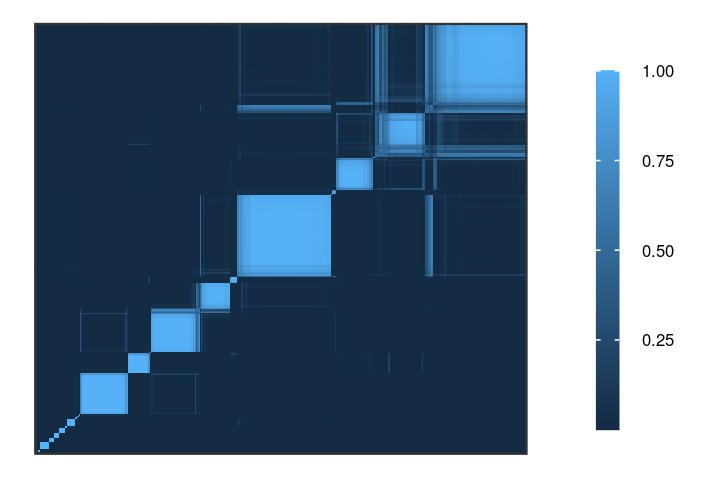
\includegraphics[width=0.588\linewidth,height=0.470\linewidth]{figure/gene_initial_coclustering-1} 

}

\caption[The inferred co-clustering matrix of gene expressions at $\alpha_0 = 6.$ ]{The inferred co-clustering matrix of gene expressions at $\alpha_0 = 6.$ }\label{fig:gene_initial_coclustering}
\end{figure}


\end{knitrout}













